\documentclass[12pt]{article}
\usepackage{graphicx}
\usepackage{geometry}
\usepackage{fancyhdr}
\usepackage{indentfirst}
\geometry{margin=1in}
\setlength{\parskip}{0.6em}
\setlength{\parindent}{1.5em}

\pagestyle{fancy}
\fancyhf{}
\fancyhead[L]{Dental Prophylaxis Chatbot}
\fancyfoot[C]{\thepage}

\title{Dental prophylaxis chatbot - Project CatchUp \\ \large Systems Analysis \\ \large Semester 2024-III}
\author{Cesar Augusto Pulido Cuervo \and Catalina Ariza Ardila}
\date{}

\begin{document}

\maketitle

\section*{System}

The dental prophylaxis is a very extensive subject, although it may not seem so at first. Prophylaxis refers to measures taken to prevent medical conditions that may occur. Dental prophylaxis is a odontology branch that include medications, cleanings and treatments that are aimed at preventing dental infections, illnesses, or other health problems before they arise.

Multiple elements of the dental prophylaxis system cooperate to guarantee the best possible oral health. The first step in the system is patient care, which includes brushing, flossing, and mouthwash as necessary practices to keep teeth clean and prevent dental diseases. Professional practices including fluoride treatment, dental sealants, and regular cleanings by a dentist support these measures. Dental sealants function as protective barriers, keeping food and germs from building up in sensitive places, while fluoride helps to strengthen teeth and lower the chance of cavities.

When combined, these preventive steps ensure improved oral health status by addressing common oral health issues such as periodontal diseases and cavities as shown in Figure \ref{fig:system}. The feedback loop illustrates how dentist interventions combined with routine updates to a patient's medical history and supplies lead to ongoing improvements in oral care techniques.

\begin{figure}[htbp]
\centerline{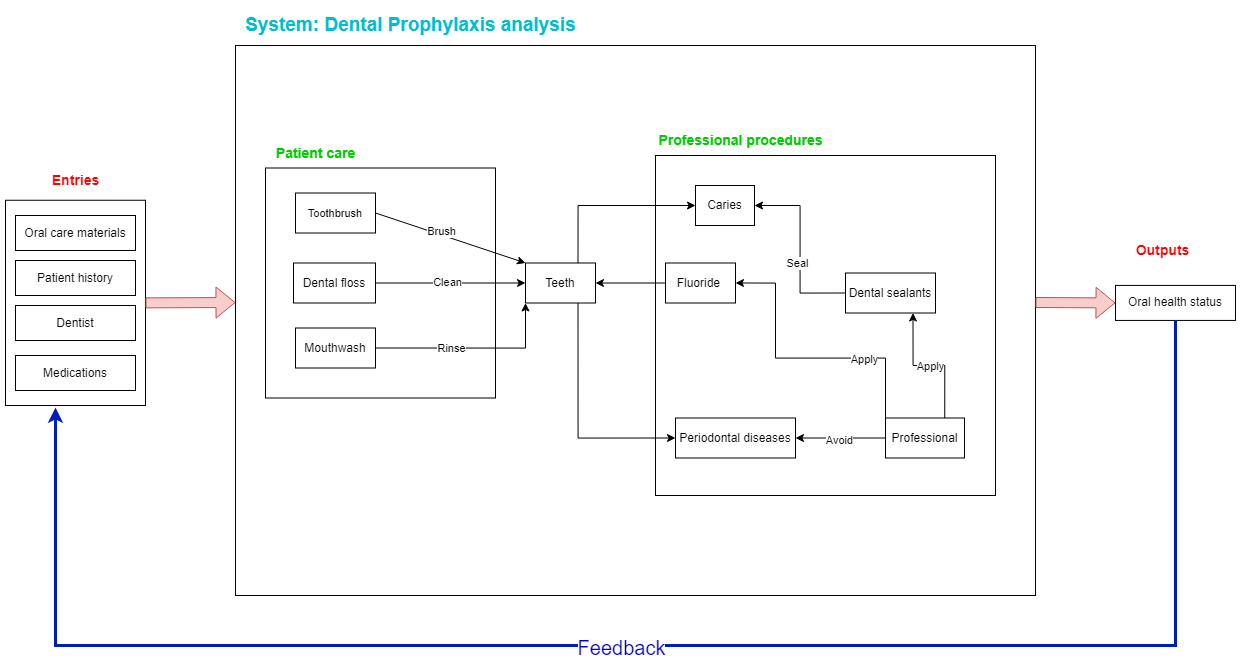
\includegraphics[width=0.96\textwidth]{figures/system.png}}
\caption{Dental prophylaxis system.}
\label{fig:system}
\end{figure}

\section*{Bounding}
In defining the boundaries of the system, recognizing the vast scope of odontology as a field was important. Owing to its breadth, attention was given to the specialty of prophylaxis, which includes oral disease prevention strategies. Daily routines like eating habits have a big impact on dental health, but adding these aspects would make the system more complex and broaden its use needlessly. Because of this, the system is designed with the specific goal of focusing only on the professional interventions and basic self-care with dental health materials associated with dental prophylaxis, making it possible to avoid oral illnesses in a more efficient and effective manner.

The following aspects are the inputs of the system:
\begin{itemize}
    \item \textbf{Oral care materials: }What the patient have for them dental self-care.
    \item \textbf{Patient history: }Previous treatments, allergies or any ongoing medical conditions.
    \item \textbf{Dentist: }What professional or institution is attending the patient, their tools, the quality of the patient's care.
    \item \textbf{Medications: }Pharmaceutical products that preserve oral health.
\end{itemize}
As the output is the health status, this feedback will lead to what medications the patient should take or if the patient's history has been updated.

\section*{Chaotic effects}
\subsection*{Snowball}
The snowball effect apears when in a small issue with an element escalates into a major problem. In the prophylaxis system, this can ocurr when:

\textbf{Improper brushing $\rightarrow$ Excess plaque $\rightarrow$ Cavities form $\rightarrow$ Oral diseases}

Is very common in many patients this progression from a minor problem, if unchecked, can lead to significant dental problems.

\subsection*{Domino}
The domino effect appears when a vulnerable element of the system is affected, causing a chain that involve various parts of the system. In this system, it can appear as follows:

\textbf{Untreated cavities + No flossing $ \rightarrow $ Toothache $ \rightarrow $ Periodontal diseases}


\end{document}
